% !TeX program = pdfLaTeX
\documentclass[12pt]{article}
\usepackage{amsmath}
\usepackage{graphicx,psfrag,epsf}
\usepackage{enumerate}
\usepackage{natbib}
\usepackage{textcomp}
\usepackage[hyphens]{url} % not crucial - just used below for the URL
\usepackage{hyperref}

%\pdfminorversion=4
% NOTE: To produce blinded version, replace "0" with "1" below.
\newcommand{\blind}{0}

% DON'T change margins - should be 1 inch all around.
\addtolength{\oddsidemargin}{-.5in}%
\addtolength{\evensidemargin}{-.5in}%
\addtolength{\textwidth}{1in}%
\addtolength{\textheight}{1.3in}%
\addtolength{\topmargin}{-.8in}%

%% load any required packages here



% tightlist command for lists without linebreak
\providecommand{\tightlist}{%
  \setlength{\itemsep}{0pt}\setlength{\parskip}{0pt}}



\usepackage[dvipsnames]{xcolor} % colors
\newcommand{\ear}[1]{{\textcolor{blue}{#1}}}
\newcommand{\svp}[1]{{\textcolor{RedOrange}{#1}}}
\newcommand{\rh}[1]{{\textcolor{Green}{#1}}}
\usepackage[capitalise]{cleveref}
\newcommand\pcref[1]{(\cref{#1})}

\begin{document}


\def\spacingset#1{\renewcommand{\baselinestretch}%
{#1}\small\normalsize} \spacingset{1}


%%%%%%%%%%%%%%%%%%%%%%%%%%%%%%%%%%%%%%%%%%%%%%%%%%%%%%%%%%%%%%%%%%%%%%%%%%%%%%

\if0\blind
{
  \title{\bf `You Draw It' Implementation of visually fitted trends with
\texttt{r2d3}}

  \author{
        Emily A. Robinson 1 \\
    Department of Statistics, University of Nebraska-Lincoln\\
     and \\     Reka Howard 2 \\
    Department of Statistics, University of Nebraska-Lincoln\\
     and \\     Susan VanderPlas 3 \\
    Department of Statistics, University of Nebraska-Lincoln\\
      }
  \maketitle
} \fi

\if1\blind
{
  \bigskip
  \bigskip
  \bigskip
  \begin{center}
    {\LARGE\bf `You Draw It' Implementation of visually fitted trends
with \texttt{r2d3}}
  \end{center}
  \medskip
} \fi

\bigskip
\begin{abstract}
How do statistical regression results compare to intuitive, visually
fitted results? Fitting lines by eye through a set of points has been
explored since the 20th century. Common methods of fitting trends by eye
involve maneuvering a string, black thread, or ruler until the fit is
suitable, then drawing the line through the set of points. In 2015, the
New York Times introduced an interactive feature, called `You Draw It,'
where readers are asked to input their own assumptions about various
metrics and compare how these assumptions relate to reality. This
research is intended to implement `You Draw It', adapted from the New
York Times, as a way to measure the patterns we see in data.
\emph{(116/200 words)}
\end{abstract}

\noindent%
{\it Keywords:} graphics, user interaction, regression
\vfill

\newpage
\spacingset{1.45} % DON'T change the spacing!

\hypertarget{introduction}{%
\section{Introduction}\label{introduction}}

Our visual system is naturally built to look for structure and identify
patterns. For instance, points going down from left to right indicates a
negative correlation between the \(x\) and \(y\) variables. How can we
compare our intuitive visual sense of patterns to those determined by
statistical methods?

\hypertarget{testing-statistical-graphics}{%
\subsection{Testing Statistical
Graphics}\label{testing-statistical-graphics}}

Graphical tests are useful for studying the perception of statistical
graphs. Studies might ask participants to identify differences in
graphs, read information off of a chart accurately, use data to make
correct real-world decisions, or predict the next few observations. All
of these types of tests require different levels of use and manipulation
of the information being presented in the chart.

Efforts in the field of statistical graphics have developed graphical
testing tools and methods. Through experimentation, graphical testing
methods allow researchers to conduct studies geared at understanding
human ability to conduct tasks related to the perception of statistical
charts such as differentiation, prediction, estimation, and
extrapolation. The advancement of graphing software provides the tools
necessary to develop new methods of testing statistical graphics.

\hypertarget{fitting-trends-by-eye}{%
\subsection{Fitting Trends by Eye}\label{fitting-trends-by-eye}}

Initial studies in the 20th century explored the use of fitting lines by
eye through a set of points
\citep{finney1951subjective, mosteller1981eye}. Common methods of
fitting trends by eye involved maneuvering a string, black thread, or
ruler until the fit is suitable, then drawing the line through the set
of points. Recently, \citet{ciccione2021can} conducted a comprehensive
set of studies investigating human ability to detect trends in graphical
representations from a psychophysical approach.

In 2015, the New York Times introduced an interactive feature, called
`You Draw It' \citep{aisch2015you}, where readers input their own
assumptions about various metrics and compare how these assumptions
relate to reality. The New York Times team utilizes Data Driven
Documents (D3) that allows readers to predict these metrics through the
use of drawing a line on their computer screen with their mouse.

\hypertarget{research-objectives}{%
\subsection{Research Objectives}\label{research-objectives}}

The goal of this research is to implement `You Draw It', adapted from
the New York Times feature, as a way to measure the patterns we see in
data. Here, we provide technical details of the software development,
utilizing interactive graphics in R. We then share results from our
study which validates `You Draw It' as a method for graphical testing
and apply an appropriate data analysis method to the participant data.

\hypertarget{development}{%
\section{Development}\label{development}}

\hypertarget{you-draw-it-task}{%
\subsection{`You Draw It' Task}\label{you-draw-it-task}}

Users are shown an interactive scatter-plot
(\cref{fig:you-draw-it-example}) along with the prompt, ``Use your mouse
to fill in the trend in the yellow box region.'' The yellow box region
moves along as the user draws their trend-line, providing a visual cue
which indicates where the user still needs to complete a trend line.
After the entire domain has been visually estimated or predicted, the
yellow region disappears, indicating the participant has completed the
task. Visit \href{https://bit.ly/3zHnlgp\%7D}{bit.ly/3zHnlgp} for a test
applet.

\hypertarget{source-code}{%
\subsection{Source Code}\label{source-code}}

Data Driven Documents (D3), a JavaScript-based graphing framework that
facilitates user interaction, is used to create the `You Draw It'
visual. A challenge of working with D3 is the environment necessary to
display the graphics and images. The \texttt{r2d3} package
\citep{r2d3pkg} provides an efficient integration of D3 visuals into R
HTML formats. We integrate the D3 visual source code into an R shiny
\citep{shinypkg} application in order to allow for user interaction and
data collection.

We conduct all data simulation and processing in R and output two data
sets - \emph{point data} and \emph{line data} - containing (\(x\),
\(y\)) coordinates corresponding to either a simulated point or fitted
value predicted by a statistical model respectively. Then, the
\texttt{r2d3} package converts the data sets in R to JSON to be
interpreted by the D3.js code. We define functions in D3.js to draw the
initial plot and set up drawable points for the user drawn line. Drag
events in D3.js are utilized to react to observe and react to user
input. Shiny Messages are used to communicate the user interaction
between the D3 code and the R environment. The plot is then rendered and
updated on user interaction into the R shiny application with the
\texttt{RenderD3} and \texttt{d3Output} functions.

Parameters for aesthetic design choices are defined in a list of options
and \texttt{r2d3} passes these to the D3.js code. For instance, we can
specify the buffer space allowed for the \(x\) and \(y\) axes to avoid
users to anchor their lines to the axes limits.

For \texttt{D3.js} source code, visit
\href{https://bit.ly/3teA3lM}{bit.ly/3teA3lM}.

\begin{figure}

{\centering 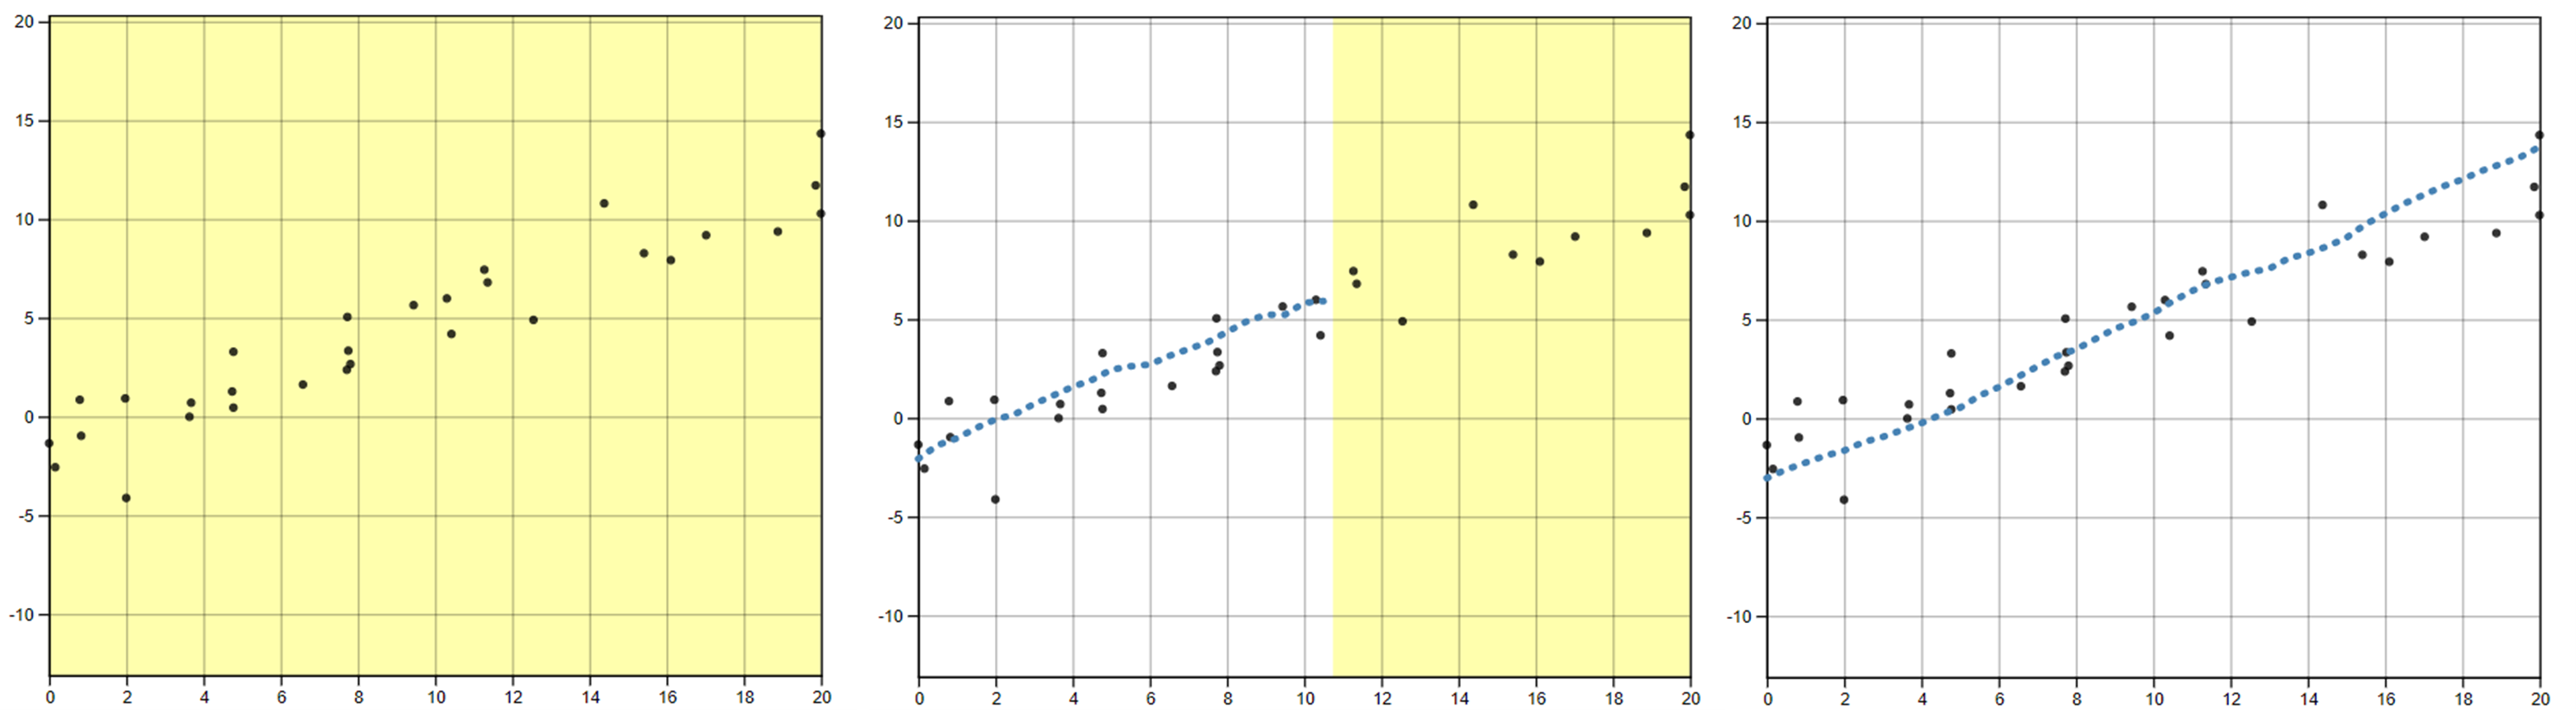
\includegraphics[width=1\linewidth]{images/ydi-stimuli} 

}

\caption{'You Draw It' interaction task plot as shown to user. \textbf{Left:} illustrates what user first sees with the prompt \textit{`Use your mouse to fill in the trend in the yellow box region.'} \textbf{Middle:} illustrates what the user sees while completing the task. \textbf{Right:} illustrates the users finished trend line.}\label{fig:you-draw-it-example}
\end{figure}

\hypertarget{application}{%
\section{Application}\label{application}}

\hypertarget{tool-validation}{%
\subsection{Tool Validation}\label{tool-validation}}

We conducted a study in order to validate `You Draw It' as a method for
graphical testing, comparing results to the less technological method
utilized in \citet{mosteller1981eye}. Results from our study were
consistent with those found in the previous study; when shown points
following a linear trend, participants tended to fit the slope of the
first principal component over the slope of the least-squares regression
line. This trend was most prominent when shown data simulated with
larger variances. This study reinforces the differences between
intuitive visual model fitting and statistical model fitting, providing
information about human perception as it relates to the use of
statistical graphics.

\hypertarget{data-analysis}{%
\subsection{Data Analysis}\label{data-analysis}}

Feedback data from conducted studies are collected and stored in a
database for analysis. Within the collected feedback data, we know the
simulated data points, the predicted values from the statistical model,
and the predicted values from the user drawn line. In our initial
studies, a unique data set was simulated independently for each
participant. Therefore, we evaluate the accuracy of the user drawn line
by observing the deviation, vertical residuals, between the user drawn
line and the predicted values from the statistical model. We use a
Generalized Additive Mixed Model (GAMM) to model the vertical residuals
in order to statistically compare visually fitted trends to actual
metrics, simulated data models, or statistical regression results. A
benefit of using a GAMM is the estimation of smoothing splines, allowing
for flexibility in the residual trend.

\hypertarget{future-work}{%
\section{Future Work}\label{future-work}}

In this work, we implemented and validated `You Draw It' as a way to
measure the patterns we see in data. We demonstrated the use of
generalized additive models to statistically model participant data.
While technical details of the development process are presented here,
we intend to create an R package designed for easy implementation of
`You Draw It' task plots in order to make this tool accessible to other
researchers. Further investigation is necessary to implement this method
real data in order to facilitate scientific communication.

\bibliographystyle{agsm}
\bibliography{bibliography.bib}


\end{document}
